\chapter{Aritmetika a teória čísel}

\begin{example}
	Vypočítaj $1,5^2 + 1,6^2 + 1,7^2$.
\end{example}

\begin{example}
	Mesačník o zdravej výžive stojí 2,90€. Pán Milan si objednal ročné predplatné, zaplatil zaň 29,50€. Koľko eur ušetril kúpou predplatného.
\end{example}

\begin{example}
	Číselná os na obrázku je zobrazená na 8 zhodných sekov. Bod A je obrazom reálneho čísla. Uveď toto číslo ako zlomok v základnom tvare.
	\begin{center}
		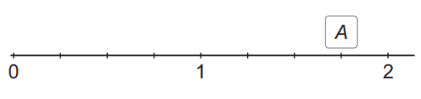
\includegraphics{assets/os1.png}
	\end{center}
\end{example}

\begin{example}
	Otec nechal synovi nasledujúci odkaz: „Ak chceš vedieť heslo na wifi, usporiadaj čísla od najmenšieho po najväčšie.“ \\
	$\frac{4}{3} = M$, $\frac{5}{4} = S$, $1,4 = P$, $1,5 = L$
	Ktoré heslo je správne?
	\begin{enumerate}
		\item LPMS
		\item MSPL
		\item PSLM
		\item SMPL
	\end{enumerate}
\end{example}

\begin{example}
	Na číselnej osi je vyznačený obraz čísla a. \\
	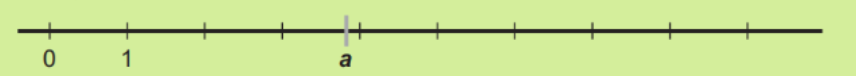
\includegraphics{assets/os2.png}\\
	Ktoré z uvedených piatich vzťahov platí pre číslo a?
	\begin{enumerate}
		\item $a - 6 > 0$
		\item $4 - a > 0$
		\item $5 - a < 0$
		\item $a - \frac{16}{3} < 0$
		\item $-1 - a < 0$
	\end{enumerate}
\end{example}

\begin{example}
	Na číselnej osi sú body A, B, C obrazmi reálnych čísel. Vypočítaj hodnotu výrazu A + B - C a výsledok zapíš v tvare desatinného čísla.\\
	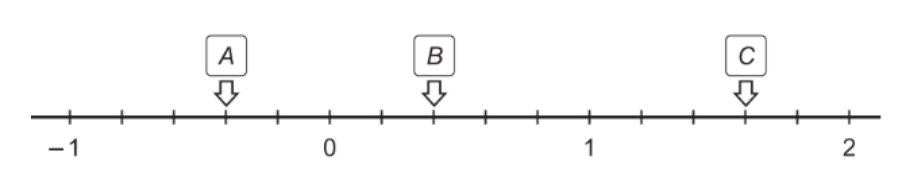
\includegraphics{assets/os3.png}
\end{example}

\begin{example}
	Na číselnej je vyznačených šedť rovnako dlhých úsekov. Bod A je obrazom reálneho čísla. Zapíš toto číslo ako zlomok v základnom tvare. \\
	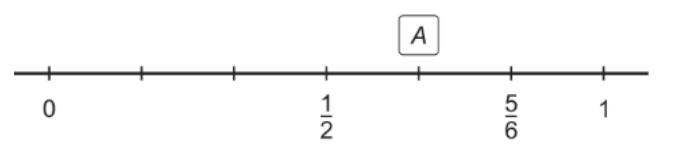
\includegraphics{assets/os4.png}
\end{example}

\begin{example}
	Desiati priatelia sa dohodli, že si objednajú pizze spolu, aby využili akciu, kde dostanú každú štvrtú pizzu zadarmo. Jedna pizza stojí 6€. Koľko eur ich vyšla 1 pizza v priemere, ak si objednali 10 pízz. Výsledok uveď s presnosťou na 2 desatinné miesta.
\end{example}

\begin{example}
	Ktorá z nasledujúcich nerovností platí? \\
	Nerovnosť 1: \fbox{$3^2 > 2^3$}. Nerovnosť 2: \fbox{$(-3)^2 < (-2)^3$}.\\
	\begin{enumerate}
		\item Platí len nerovnosť 1.
		\item Platí len nerovnosť 2.
		\item Platia obe nerovnosti.
		\item Neplatí ani jedna nerovnosť.
	\end{enumerate}
\end{example}

\begin{example}
	Číslo na nazýva dokonalé, ak je súčet jeho deliteľov okrem seba samého rovný tomuto číslu.\\
	Napríklad číslo 28 je dokonalé. Súčet jeho deliteľov 1, 2, 4, 7, 14 je 28. \\
	Ktoré z nasledujúcich čísel je tiež dokonalé?
	\begin{enumerate}
		\item 14
		\item 12
		\item 8
		\item 6
	\end{enumerate}
\end{example}

\begin{example}
	Riadky tabuľky sú označené písmenami R, S, T a stĺpce číslami 1, 2, 3. Do výrazu \textbf{R2 - S3 + T1} dosaď príslušné čísla a vypočítaj jeho hodnotu. \\
	\begin{center}
		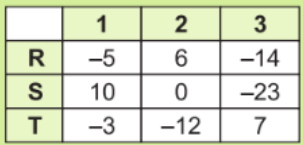
\includegraphics{assets/tab.png}
	\end{center}
	
\end{example}

\begin{example}
	Na farme chovajú 110 kusov hydiny (sliepky, morky, kačky a husi). Sliepky predstavujú polovicu. moriek je 10 a kačiek je o 7 viac ako husí. Koľko husí chovajú na farme?
\end{example}

\begin{example}
	Koľkokrát je číslo $5 \cdot 10^5$ väčšie ako číslo $125 \cdot 10^3$?
\end{example}

\begin{example}
	Vypočítaj dve tretiny z troch štvrtín. Výsledok zapíš ako zlomok v základnom tvare.
\end{example}

\begin{example}
	Traja súrodenci si objednali pizzu. Miška zjedla štvrtinu z pizze. Lenka zjedna tretinu zo zyšku a Patrik zjedol polovicu z toho, čo nechala Lenka. Zvyšok si nechali zabaliť domov. Akú časť pizze im zabalili? Výsledok zapíšte ako zlomok v základnom tvare. 
\end{example}

\begin{example}
	Pavlína má stovky svojich fotografií z dovolenky uložené na pamäťových kartách. Všetky fotografie dala vytlačiť. V tabuľke sú uvedené počty fotografií a ceny za ich vytlačenie. Koľko eur zaplatila Paulína za vytlačenie všetkých svojich fotografií s rozmermi $10 \times 15$ cm.
	
	\begin{center}
		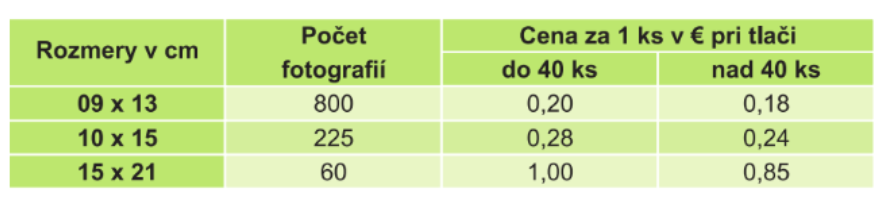
\includegraphics{assets/fotky.png}
	\end{center}
\end{example}

\begin{example}
	Vypočítaj a výsledok zapíš v tvare desatinného čísla.\\ $\frac{3}{4} -1\frac{2}{5} + 0,5$.
\end{example}

\begin{example}
	Máme číslo A = 753 672. Vypočítaj rozdiel čísla A zaokrúhľeného na stovky a čísla A zaokrúhleného na desaťtisíce.
\end{example}

\begin{example}
	Vypočítaj $\frac{1}{3} + \frac{1}{3} \cdot \frac{1}{3} + \frac{1}{3}$.\\
	\begin{enumerate}
		\item $0.\overline{8}$
		\item $0.\overline{7}$
		\item $0.\overline{5}$
		\item $0.\overline{4}$
	\end{enumerate}
\end{example}

\begin{example}
	Vyber mocninu, ktorá má najväčšiu hodnotu.
	\begin{enumerate}
		\item $5^2$
		\item $4^3$
		\item $3^4$
		\item $2^5$
	\end{enumerate}
\end{example}

\begin{example}
	Vypočítaj $800 - 700 \div 2 + 100 \cdot 14.67$.
\end{example}

\begin{example}
	Na číselnej osi sú zobrazené M, A, V. Vypočítaj M + A + V. \\
	\begin{center}
		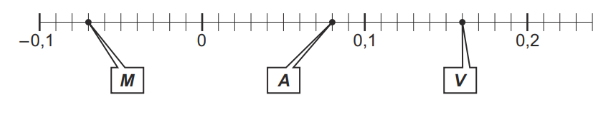
\includegraphics{assets/os5.png}
	\end{center}
\end{example}

\begin{example}
	Vypočítaj $(-0,7)^2 \cdot 10^2 + (-0,2 \cdot 10)^3$.
\end{example}

\begin{example}
	Z čísel uvedených na kartičkách sčítaj najmenjšie a najväčšie číslo.\\
	\begin{center}
		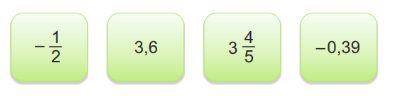
\includegraphics{assets/karticky.png}
	\end{center}
\end{example}

\begin{example}
	Pri tovare \textbf{B} bola ponuka: \textbf{Ak si zoberiete 6 kusov, zaplatíte len za 4 kusy}. Jeden kus tohoto tovaru stojí 7€. Mária si zobrala 31 kusov tohoto tovaru. Koľko eur zaplatila za tovaru?
\end{example}

\begin{example}
	Vypočítaj hodnotu výrazu $\frac{1}{4} + \frac{3}{2} - \frac{5}{6}$. Výsledok uveď ako desatinné číslo na dve desatinné miesta.
\end{example}

\begin{example}
	Vypočítaj súčin výrazov A a B. \\
	$A = 10 - (9 - 8) - (6 - 7)$\\
	$B = 4 \cdot 10^2 + 5 \cdot 10 + 9$
\end{example}

\begin{example}
	Ktoré číslo je na číslenej osi rovnako vzdialené od čísel 299 a 1051?
\end{example}

\begin{example}
	Anka si na výlet kúpila 1,5 litra minerálky. Tri pätiny z nej vypila. Vyber pravdivé tvrdenia. \\
	\begin{enumerate}
		\item Vypila menej ako polovicu.
		\item Zostalo jej 6 dl minerálky.
		\item Vypila viac ako jeden liter minerálky.
		\item Zostali jej dve tretiny minerálky.
	\end{enumerate}
\end{example}

\begin{example}
	V mise bolo 100 sliviek. Igor si z nej zobral 2 slivky a Viera si zobrala $\frac{4}{7}$ zo zvyšku. Koľko sliviek zostalo v mise?
\end{example}

\begin{example}
	Kamaráti Filip a Tibor počítali príklady z matematiky. \\
	Filip: $3 - 12 \cdot 5 -18 = -75$\\
	Tibor: $40 - (90 - 	55) \div 5 = 1$
\end{example}

\begin{example}
	Vypočítaj $\frac{1}{2} + \frac{2}{3} \cdot \frac{3}{4} - \frac{4}{5} \div \frac{6}{5}$. Výsledok uveď ako zlomok v základnom tvare.
\end{example}

\begin{example}
	Adam a Eva počítali príklady.  \\
	Adam uviedol, že výsledok príkladu $0 - (-2)^3$ je 8. \\
	Eva uviedla, že výsledok príkladu $(-3)^2 - 1$ je -8. \\
	Vyber pravdivé tvrdenie.
	\begin{enumerate}
		\item Obaja uviedli správne výsledky.
		\item Len Adam uviedol správny výsledok.
		\item Len Eva uviedla správny výsledok.
		\item Ani jeden neuviedol správny výsledok.
	\end{enumerate}
\end{example}

\begin{example}
	Dvojnásobok čísla $4^2$ odpočítaj od čísla $\sqrt{\frac{9}{16}}$. Výsledok uveď ako zlomok v základnom tvare.
\end{example}